%
% Angepasste FOM Seminarvorlage
%
\documentclass[12pt,a4paper,listof=totoc,bibliography=totoc]{scrartcl}

\usepackage[english]{babel}			% englische Namen/Umlaute
\usepackage[utf8]{inputenc}	    	% Zeichensatzkodierung
\usepackage{silence}
 \WarningFilter{scrartcl}{Usage of package `fancyhdr'}
 \WarningFilter{scrartcl}{Usage of package `parskip'}
\usepackage{fancyhdr}
\usepackage{graphicx}               % Einbinden von Bildern
\usepackage[hidelinks]{hyperref}	% Klickbare Verweise und \autoref{label}
\usepackage[intoc]{nomencl}
\usepackage{setspace}
\usepackage{parskip}
\usepackage{caption}
\usepackage{float}
\usepackage{listings}
\usepackage{scrhack}
\usepackage{geometry}
 \geometry{a4paper, left=40mm, right=20mm, top=40mm, bottom=20mm}
\renewcommand{\familydefault}{\sfdefault}
\renewcommand{\ttdefault}{pcr}
\renewcommand{\lstlistlistingname}{Listings}
\renewcommand{\lstlistingname}{Listing}
\usepackage{float}
\floatstyle{plaintop}
\restylefloat{table}

% Bildueberschrift oben und rechtsbuendig
\captionsetup{labelfont=bf, textfont=bf}
\captionsetup{justification=raggedright,singlelinecheck=false}

% Blocksatz
\def\justify{%
  \rightskip=0pt
  \spaceskip=0pt
  \xspaceskip=0pt
  \relax
}

%
%	Hier werden Titel, Bearbeiter und das Datum eingetragen
%
\newcommand\svthema{Awareness}
\newcommand\svperson{Christian Frank (\#473088)}
\newcommand\svdatum{\today}
\newcommand\lvname{Verhandlungstechniken}
\newcommand\lvtyp{Sommerkonferenz Sopron 2025}
\newcommand\lvinst{FOM - Hochschule für Oekonomie \& Management}
\newcommand\lvbetr{Prof. Dr. Mónika Cseresznyák}

\hypersetup{ % Thema und Author in die Meta-Daten der PDF
  pdftitle={\svthema}, 
  pdfauthor={Christian Frank},
  pdfsubject={Awareness},
  pdfkeywords={Awareness, NVC, GFK, Conflict}
}

\begin{document}

% Titel
\title{ \huge\textbf{\svthema} }
\author{ {\svperson} \\ \svdatum }
\date{ \normalsize \centering 
\includegraphics[width=0.3\textwidth]{FOM}\\ {\lvname} \\ {\lvbetr} \\ {\lvinst} \\ {\lvtyp} }

% Seitennummer oben
\pagestyle{fancy}
\fancyhf{}
\fancyhf[ch]{\thepage}
\renewcommand\headrulewidth{0pt}

\maketitle
\thispagestyle{empty} % laesst die Seitennummer auf der Titelseite verschwinden
\pagenumbering{Roman}

\begin{abstract}
In this paper, we will examine the role Nonviolent Communication can play in conflict prevention and resolution. We will focus on practical implications for Awareness Teams in activist setups and events.

\end{abstract}

\vfill
\begin{figure}[h]
    \centering
    
\includegraphics[]{CC-BY}
\end{figure}

This work is licensed under the Creative Commons Attribution 4.0 International License. To view a copy of this license, visit http://creativecommons.org/licenses/by/4.0/ or send a letter to Creative Commons, PO Box 1866, Mountain View, CA 94042, USA.

\cleardoublepage

\tableofcontents			% Inhaltsverzeichnis
\cleardoublepage

% \listoffigures				% Abbildungsverzeichnis
% \cleardoublepage

% \listoftables               % Tabellen
% \cleardoublepage

% \lstlistoflistings			% Codeverzeichnis
% \cleardoublepage

%
% Abkuerzungsverzeichnis
%
\makenomenclature
\renewcommand{\nomname}{List of Abbreviations}

\nomenclature{\textbf{APA}}{American Psychological Association}
\nomenclature{\textbf{NVC}}{Non-Violent Communication}

\printnomenclature[1.5in]          % Abkuerzungsverzeichnis
\cleardoublepage

\pagenumbering{arabic}
\setcounter{page}{4}

%
%	Einfuehrung
%

\pagebreak
\section{Introduction}

\onehalfspacing

\subsection{Non-Violent Communication}

Nonviolent Communication (NVC) is a communication process created by psychologist Marshall B. Rosenberg.

Rosenberg believes that every communication, both verbal and nonverbal, is a form of exchange and negotiation between partners and that we can perform these exchanges with or without compassion.

NVC assumes that compassionate communication yields different results than uncompassionate communication and that these differences have a significant impact on both individual and societal levels.\footnote{See \textit{Rosenberg, M. (2015)}: Nonviolent Communication. \cite{rosenbergNvc}}

Or, as Paul Watzlawik put it, "One cannot not communicate." \footnote{\textit{Watzlawik, P. (1972)}: Pragmatics of Human Communication. \cite{watzlawick}}

\subsection{Awareness}

Awareness in the context of a social setting means being attentive to situations where a person's boundaries and sense of security are crossed,

Awareness work is based on the understanding that spaces are created differently by people who are in them. We always want to treat each other respectfully so that everyone feels as safe as possible, and we want to be attentive and sensitive to individual boundaries and needs.

Awareness work is always partisan, and boundary crossings are defined by those affected themselves.\footnote{See \textit{Fluid (2022)}: Fluid Awareness Konzept. \cite{fluidAware}}

\subsection{Research Question \& Method}

This paper will examine the use of NVC for conflict resolution. To do this, we will evaluate the case of an Awareness concept in activist settings and events.\footnote{See \textit{McCombes, S. (2019)}: What is a Case Study. \cite{caseScribbr}}

The goal of this paper is to establish whether NVC is a valuable tool for conflict resolution and awareness in group settings.

\subsection{Gender-neutral Pronouns}

Our society is becoming more open, inclusive, and gender-fluid, and now I think it's time to think about using gender-neutral pronouns in scientific texts, too. Two well-known researchers, Abigail C. Saguy and Juliet A. Williams, both from UCLA, propose to use the singular they/them instead: "The universal singular they is inclusive of people who identify as male, female or nonbinary." \footnote{\textit{Saguy, A. (2020)}: Why We Should All Use They/Them Pronouns. \cite{pronouns}} The aim is to support an inclusive approach in science through gender-neutral language. 

In this paper, I'll attempt to follow this suggestion and invite all my readers to do the same for future articles. Thank you!

If you're not sure about the definitions of gender and sex and how to use them, have a look at the definitions\footnote{See \textit{APA (2021)}: Definitions Related to Sexual Orientation. \cite{apaDefinitions}} by the American Psychological Association.

\subsection{Climate Emergency}

As Professor Rahmstorf puts it: "Without immediate, decisive climate protection measures, my children currently attending high school could already experience a 3-degree warmer Earth. No one can say exactly what this world would look like—it would be too far outside the entire experience of human history. But almost certainly, this earth would be full of horrors for the people who would have to experience it." \footnote{\textit{Rahmstorf, A. (2024)}: Climate and Weather at 3 Degrees More. \cite{3dgreesMore}}


%
%	Begrifflichkeiten
%

\pagebreak
\section{Nonviolent Communication}

\onehalfspacing

\subsection{Philosophical Background}

Dialectical materialism is a philosophical movement developed by Karl Marx and Friedrich Engels that explains the world in a materialistic manner, i.e., starting from material conditions.\footnote{See \textit{MIA (2022)}: Encyclopedia of Marxism. \cite{diaMat}}

It uses the dialectical method, which views contradictions and change as the driving force behind development. There are no direct "business models" in the sense of today's economic concepts that can be derived from dialectical materialism. However, certain principles of dialectical materialism can be applied to the analysis of business models to understand their contradictions and potential for development.

The dialectical method helps to analyze the development of a business model and to understand how quantitative changes (e.g., growth) can lead to qualitative leaps (e.g., new business areas).

A business model can also be negated by external influences (e.g., technological innovations) or internal developments (e.g., strategic realignment) and replaced by a new one.

\subsection{Concepts}

Concepts

\subsection{Jackal and Giraffe}

Jackal and Giraffe

\subsection{Communication Steps}

Communication Steps

\begin{figure}[H]
\centering
\caption {Four Steps}
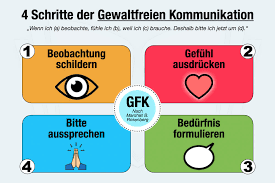
\includegraphics[width=\linewidth]{images/images.png}
\label{fig:fourSteps}
\end{figure}

\begin{figure}[H]
\centering
\caption {Examples}
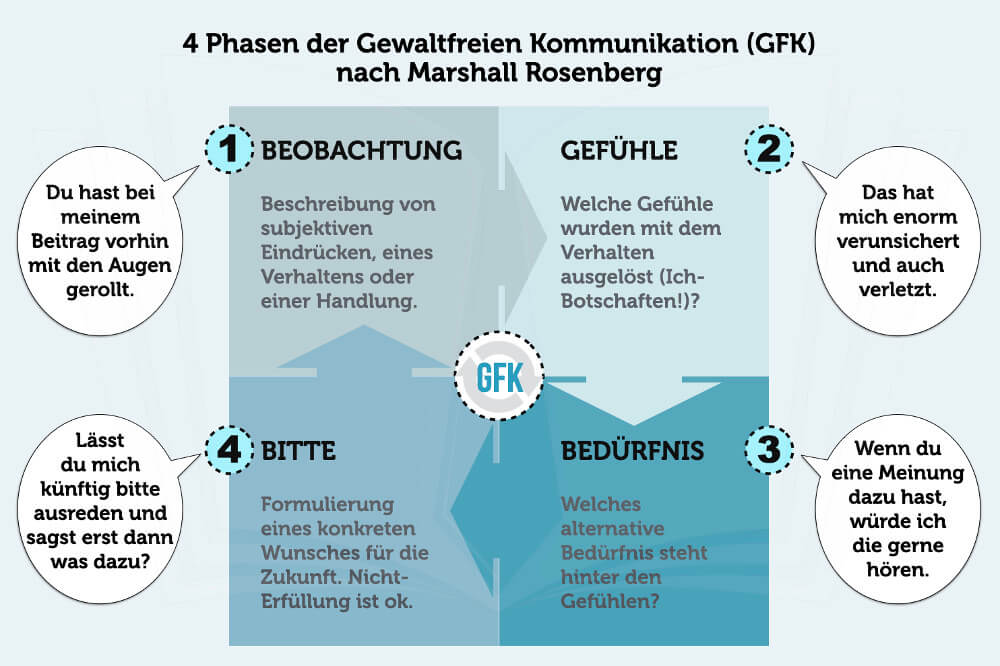
\includegraphics[width=\linewidth]{images/Gewaltfreie-Kommunikation-Beispiele.jpeg}
\label{fig:examples}
\end{figure}


%
%	Theorieteil
%

\pagebreak
\section{Conflicts}

\onehalfspacing

\subsection{Definition}

Conflict as a social phenomenon is a complex aspect of human interaction that extends far beyond individual disagreements.

Generally speaking, a conflict emerges when two or more parties perceive their interests, values, needs, or goals as incompatible or mutually exclusive. It's an inherent feature of social life, arising wherever people interact.

Potential structural sources of social conflict are:

\begin{itemize}
    \item Resource competition
    \item (Gender) Role conflicts
    \item Value differences
    \item Power imbalances\footnote{See \textit{Omelaenko, N. (2021)}: Conflict As A Social Phenomenon. \cite{conflict}}
\end{itemize}

\subsection{Scenarios}

In social groups, gatherings, or events, there are a couple of possible conflict scenarios:

\begin{itemize}
    \item Miscommunication
    \item Disagreements
    \item Inappropriate/harassing behavior
    \begin{itemize}
        \item Offensive pictures (e.g., in online meetings)
        \item Unwanted (physical) contact
        \item Misogyny and other forms of hate speech
        \item Mansplaining
        \item Any other forms of (White) male dominance behavior
    \end{itemize}    
\end{itemize}

For the remainder of this paper, we will focus on inappropriate or harassing behaviour.

\subsection{Code of Conduct}

A key step in dealing with conflict is to define the boundaries of acceptable behavior up front clearly.

The most common way is to create a clear and unambiguous Code of Conduct.\footnote{See \textit{Ruby Berlin e.V. (2017)}: Berlin Code of Conduct. \cite{coc}}

The Code of Conduct should cover:

\begin{itemize}
    \item A clear and detailed definition of expected behaviour, beyond the "Be excellent to each other"
    \item A clear and detailed definition of unacceptable behavior, such as unwanted contact or unsolicited communication
    \item The consequences of unacceptable behavior, such as removal from the event
    \item Instructions on where and how to address grievances
\end{itemize}

Most large social events, such as conferences or festivals, now have a clear Code of Conduct and set boundaries on acceptable behavior.

\subsection{Awareness Team}

But even with a Code of Conduct defined, conflicts will arise.

To deal with conflicts, Awareness-Teams could be created. In the next chapter, we will explore the concept of Awareness and consider what a team might look like.

To prevent and resolve conflicts, the Awareness-Teams themselves must be able to engage and communicate without resorting to violence. The practice of nonviolent communication is an excellent basis for the work of Awareness-Teams.


%
%	Praxisbezug
%

\pagebreak
\section{Awareness-Team}

\onehalfspacing

\subsection{Implementation}

To support the Code of Conduct and assist with conflict resolution, many large events and organizations employ Awareness-Teams.\footnote{See \textit{FFF (2021)}: Awareness OG Leitfaden. \cite{fffAware}}

The roles and responsibilities of the Awareness-Team are laid out in an Awareness-Concept. This concept should be agreed upon in advance and preferably enjoys majority support.

Responsibilities could include the following tasks:

\begin{itemize}
    \item Code of conduct enforcement
    \item Safe space maintenance
    \item Incident response at gatherings
    \item Accessibility and inclusion support
    \item Harassment and discrimination prevention
    \item Anti-bullying initiatives
    \item Sexual assault prevention
\end{itemize}

The role of the team is twofold: it should create Awareness before problems occur and respond to incidents after they happen.

A key capability for the team member is the ability to de-escalate a conflict situation by communicating effectively and nonviolently.

The effectiveness of an Awareness-Team depends heavily on organizational support, a clear mandate, appropriate training, and genuine commitment of the organization to creating safer, more inclusive environments.

\subsection{Real-World Example \& Safe Word}

One of the first event agencies to embrace Awareness for their concerts and festivals was \href{https://fkpscorpio.com/}{FKP Scorpio}.

They ensured that Awareness-Teams were on-site and visible, and also introduced Safe Spaces as safe environments for anyone seeking help.

To further support this, and make access even simpler, FKP Scorpio introduced a code phrase, "Where is Panama?", that would signal staff that the person needs immediate support, without alerting bystanders or the perpetrator.\footnote{See \textit{FKP Scorpio (2023)}: Wo geht's nach Panama. \cite{panama}}

Rumours have it that the phrase was chosen as a reference to the children's book "The Trip to Panama" by Janosch.

Over the years, this concept has spread through most events. 

A similar idea is behind the international Signal for Help that alerts to violence at home.

\subsection{Conclusion}

The mindset and practice of Non-Violent Communication are key capabilities for anyone involved in Awareness Work.

A deep understanding of the shared humanity of all of us, the knowledge that all living beings strive for happiness, will make sure that the Awareness-Concept is sound and that the work of the Awareness-Team will be successful and beneficial.


%
%	Fazit
%

\pagebreak
\section{Summary}

\onehalfspacing

Non-Violent Communication, or Compassionate Communication, is a great tool to support awareness and conflict resolution processes in groups.

Based on its fundamentally humanistic approach to human interaction, NVC provides practical guidelines for establishing appreciative communication, which can help prevent conflicts from arising and support defusing conflict situations.

We demonstrated that an awareness team educated in NVC can greatly benefit large social gatherings and groups, and can recommend exploring the concepts behind NVC further.

Happy Communicating!


% Literaturverzeichnis
\cleardoublepage
\raggedright
\bibliographystyle{IEEEtranS}	% ieeetran verwenden, damit auch URLs angezeigt werden
\bibliography{seminar-lit}

\cleardoublepage
\justify
%
%	Tools (Sopron)
%

\pagebreak
\section{Tools}

\onehalfspacing

In addition to the documented references, these tools were used in creating this paper:

\begin{itemize}
    \item \href{http://www.overleaf.com}{Overleaf} to write the text
    \item \href{https://github.com/chfrank-cgn}{GitHub} for backup and version control
    \item Anthropic's \href{https://www.anthropic.com/claude}{Claude} for research
    \item \href{https://app.grammarly.com/}{Grammarly} for spellcheck and style
\end{itemize}



\cleardoublepage
\justify
%
%	Ehrenwoertliche Erklaerung
%

\pagebreak

\pagenumbering{gobble} % Keine Seitenzahlen mehr
\onehalfspacing

%-----------------------------------
% Ehrenwoertliche Erklärung
%-----------------------------------
\section*{Declaration in lieu of oath}

\par\medskip

I hereby declare that I produced the submitted paper independently, without assistance from any other party, and without using any unauthorized aids. In particular, I have marked all passages reproduced verbatim or near-verbatim from publications as quotations. Also, I declare that the submitted print version of this thesis is identical to its digital version. Furthermore, I have never presented this thesis to any examination board in its current form or any other similar version. I herewith agree that you may publish this thesis. I herewith consent to you uploading this thesis to an external contractor's server to submit it to the contractor's plagiarism detection systems. Uploading this thesis to send it to plagiarism detection systems does not constitute publication.

\par\medskip
\par\medskip

\vspace{5cm}

\begin{table}[H]
	\begin{tabular*}{\textwidth}{c @{\extracolsep{\fill}} ccccc}
		Cologne, \the\month/\the\day/\the\year \\
		\rule[0.5ex]{12em}{0.55pt} & \rule[0.5ex]{12em}{0.55pt} \\
		(Location, Date) & (Signature)
	\end{tabular*}
\end{table}


\end{document}
